\documentclass{standalone}
\usepackage[utf8]{inputenc}
\usepackage{pgfplots}
\DeclareUnicodeCharacter{2212}{−}
\usepgfplotslibrary{groupplots,dateplot}
\usetikzlibrary{patterns,shapes.arrows}
\pgfplotsset{compat=newest}
\begin{document}
% This file was created by tikzplotlib v0.9.8.
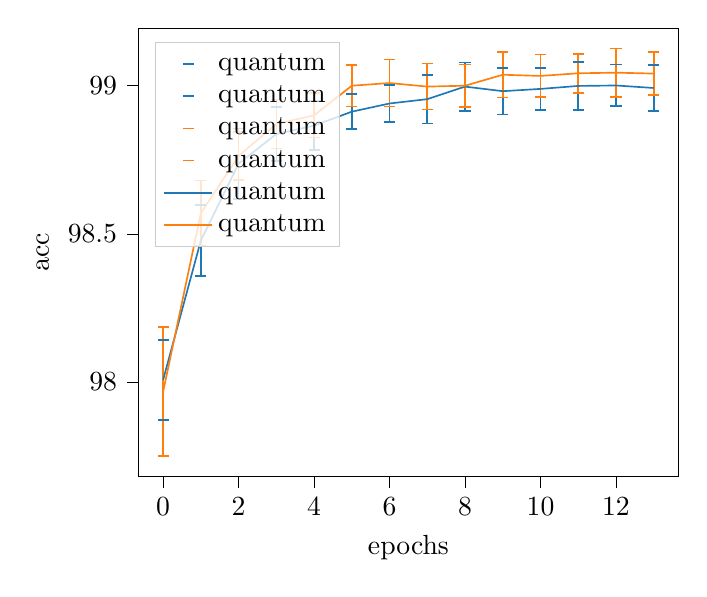
\begin{tikzpicture}

\definecolor{color0}{rgb}{0.12156862745098,0.466666666666667,0.705882352941177}
\definecolor{color1}{rgb}{1,0.498039215686275,0.0549019607843137}

\begin{axis}[
legend cell align={left},
legend style={
  fill opacity=0.8,
  draw opacity=1,
  text opacity=1,
  at={(0.03,0.97)},
  anchor=north west,
  draw=white!80!black
},
tick align=outside,
tick pos=left,
x grid style={white!69.0196078431373!black},
xlabel={epochs},
xmin=-0.65, xmax=13.65,
xtick style={color=black},
y grid style={white!69.0196078431373!black},
ylabel={acc},
ymin=97.6806278861571, ymax=99.1940572420661,
ytick style={color=black}
]
\path [draw=color0, semithick]
(axis cs:0,97.8720507945802)
--(axis cs:0,98.141795359266);

\path [draw=color0, semithick]
(axis cs:1,98.3572346007093)
--(axis cs:1,98.5981500146753);

\path [draw=color0, semithick]
(axis cs:2,98.6179282731978)
--(axis cs:2,98.8559178806483);

\path [draw=color0, semithick]
(axis cs:3,98.7450716404045)
--(axis cs:3,98.9287745134417);

\path [draw=color0, semithick]
(axis cs:4,98.7823076923077)
--(axis cs:4,98.9484615384615);

\path [draw=color0, semithick]
(axis cs:5,98.8533221861148)
--(axis cs:5,98.9712931985006);

\path [draw=color0, semithick]
(axis cs:6,98.8773655292744)
--(axis cs:6,99.0026344707256);

\path [draw=color0, semithick]
(axis cs:7,98.8721891579625)
--(axis cs:7,99.0370416112683);

\path [draw=color0, semithick]
(axis cs:8,98.9155516951286)
--(axis cs:8,99.0782944587176);

\path [draw=color0, semithick]
(axis cs:9,98.9032052331194)
--(axis cs:9,99.0598716899575);

\path [draw=color0, semithick]
(axis cs:10,98.9185786922879)
--(axis cs:10,99.0598828461736);

\path [draw=color0, semithick]
(axis cs:11,98.9177576459171)
--(axis cs:11,99.0807038925444);

\path [draw=color0, semithick]
(axis cs:12,98.9304445400114)
--(axis cs:12,99.071093921527);

\path [draw=color0, semithick]
(axis cs:13,98.9157315516016)
--(axis cs:13,99.0688838330138);

\path [draw=color1, semithick]
(axis cs:0,97.7494201296075)
--(axis cs:0,98.1845798703925);

\path [draw=color1, semithick]
(axis cs:1,98.4602730662053)
--(axis cs:1,98.6797269337948);

\path [draw=color1, semithick]
(axis cs:2,98.682)
--(axis cs:2,98.844);

\path [draw=color1, semithick]
(axis cs:3,98.788)
--(axis cs:3,98.954);

\path [draw=color1, semithick]
(axis cs:4,98.8253006024121)
--(axis cs:4,98.9746993975879);

\path [draw=color1, semithick]
(axis cs:5,98.9294308849425)
--(axis cs:5,99.0705691150575);

\path [draw=color1, semithick]
(axis cs:6,98.9298229831327)
--(axis cs:6,99.0881770168672);

\path [draw=color1, semithick]
(axis cs:7,98.9191475755034)
--(axis cs:7,99.0748524244966);

\path [draw=color1, semithick]
(axis cs:8,98.9281668600157)
--(axis cs:8,99.0718331399843);

\path [draw=color1, semithick]
(axis cs:9,98.9603123217198)
--(axis cs:9,99.1136876782801);

\path [draw=color1, semithick]
(axis cs:10,98.9611598997774)
--(axis cs:10,99.1048401002227);

\path [draw=color1, semithick]
(axis cs:11,98.9764561215673)
--(axis cs:11,99.1075438784327);

\path [draw=color1, semithick]
(axis cs:12,98.9627350013844)
--(axis cs:12,99.1252649986156);

\path [draw=color1, semithick]
(axis cs:13,98.9681371150722)
--(axis cs:13,99.1138628849278);

\addplot [semithick, color0, mark=-, mark size=2, mark options={solid}, only marks]
table {%
0 97.8720507945802
1 98.3572346007093
2 98.6179282731978
3 98.7450716404045
4 98.7823076923077
5 98.8533221861148
6 98.8773655292744
7 98.8721891579625
8 98.9155516951286
9 98.9032052331194
10 98.9185786922879
11 98.9177576459171
12 98.9304445400114
13 98.9157315516016
};
\addlegendentry{quantum}
\addplot [semithick, color0, mark=-, mark size=2, mark options={solid}, only marks]
table {%
0 98.141795359266
1 98.5981500146753
2 98.8559178806483
3 98.9287745134417
4 98.9484615384615
5 98.9712931985006
6 99.0026344707256
7 99.0370416112683
8 99.0782944587176
9 99.0598716899575
10 99.0598828461736
11 99.0807038925444
12 99.071093921527
13 99.0688838330138
};
\addlegendentry{quantum}
\addplot [semithick, color1, mark=-, mark size=2, mark options={solid}, only marks]
table {%
0 97.7494201296075
1 98.4602730662053
2 98.682
3 98.788
4 98.8253006024121
5 98.9294308849425
6 98.9298229831327
7 98.9191475755034
8 98.9281668600157
9 98.9603123217198
10 98.9611598997774
11 98.9764561215673
12 98.9627350013844
13 98.9681371150722
};
\addlegendentry{quantum}
\addplot [semithick, color1, mark=-, mark size=2, mark options={solid}, only marks]
table {%
0 98.1845798703925
1 98.6797269337948
2 98.844
3 98.954
4 98.9746993975879
5 99.0705691150575
6 99.0881770168672
7 99.0748524244966
8 99.0718331399843
9 99.1136876782801
10 99.1048401002227
11 99.1075438784327
12 99.1252649986156
13 99.1138628849278
};
\addlegendentry{quantum}
\addplot [semithick, color0]
table {%
0 98.0069230769231
1 98.4776923076923
2 98.7369230769231
3 98.8369230769231
4 98.8653846153846
5 98.9123076923077
6 98.94
7 98.9546153846154
8 98.9969230769231
9 98.9815384615385
10 98.9892307692307
11 98.9992307692308
12 99.0007692307692
13 98.9923076923077
};
\addlegendentry{quantum}
\addplot [semithick, color1]
table {%
0 97.967
1 98.57
2 98.763
3 98.871
4 98.9
5 99
6 99.009
7 98.997
8 99
9 99.037
10 99.033
11 99.042
12 99.044
13 99.041
};
\addlegendentry{quantum}
\end{axis}

\end{tikzpicture}

\end{document}